\documentclass[a4paper,utf8]{article}
\usepackage[heading,fancyhdr]{ctex}
\usepackage{amsmath,amssymb,geometry,lastpage,ulem}
\usepackage{array,tabularx,tabulary,mhchem,xspace}
\usepackage{floatrow,subfig,multirow,bigstrut}
\usepackage{siunitx,booktabs,longtable,graphicx,xfrac,nameref}
\lineskiplimit=1pt
\lineskip=3pt
\geometry{
    top=25.4mm, 
    left=25mm, 
    right=25mm, 
    bottom=25mm,
    headsep=5.9mm,
}
\ctexset{
    section = {format+=\raggedright}
}
\newcommand{\fgref}[1]{图~\ref{#1}\xspace}
\newcommand{\seqref}[1]{式~(\ref{#1})}
\newcommand{\expinfo}[7][无]{
    {\zihao{-3}\bfseries\songti
    实验名称:\uline{\hfill\mbox{#2}\hfill} \\[2.9mm]
    学\quad 号:\uline{\makebox[25mm]{#3}}\hfill
    姓\quad 名:\uline{\makebox[25mm]{#4}}\hfill
    班\quad 级:\uline{\makebox[25mm]{#5}} \\[2.9mm]
    合作者:\uline{\makebox[25mm]{#1}} \hfill
    桌\quad 号:\uline{\makebox[25mm]{#6}}\hfill\makebox[25mm+4em]{}\\[2.9mm]
    实验日期:\uline{\makebox[30mm]{#7}}\hfill\mbox{} \\[58.7mm]
    }
}
\newcommand{\pointingbox}{
    {\zihao{4}\bfseries\songti%
    实验考核\\[3mm]
    \extrarowheight=3mm
    \begin{tabularx}{150mm}{|X|X|X|X|X|}\hline
        \hfil 项目 \hfil  & \hfil 实验预习 \hfil & \hfil 实验过程 \hfil & \hfil 分析与讨论 \hfil & \hfil 总评 \hfil \\[3mm] \hline
        \hfil 评价 \hfil &  &  &  &  \\[3mm] \hline
    \end{tabularx}
    }
}
\newcommand{\derivative}[2]{\frac{\mathrm{d} #1}{\mathrm{d} #2}}
\newcommand{\thinking}[2]{\textbf{#1}\\
答:\begin{minipage}[t]{0.85\textwidth}
    #2
\end{minipage}}
\pagestyle{fancy}
\fancyhf{} \fancyhead[C]{电路基础实验} \fancyfoot[C]{\thepage~/~\pageref{LastPage}}
\newcounter{Rownumber}
\newcommand*{\Rown}{\stepcounter{Rownumber}\theRownumber}
\newcommand*{\resetRown}{\setcounter{Rownumber}{0}}
\newcommand{\qrange}[3]{\qtyrange[range-phrase = \text{$\sim$},range-units =single]{#1}{#2}{#3}}
\floatsetup[table]{capposition=top}
\newcolumntype{C}{>{\hfil}X<{\hfil}}
\renewcommand{\Nameref}[1]{\textbf{\ref{#1}~\nameref{#1}}} %导入导言
\begin{document}
\begin{center}
    {\mbox{}\\[7em]\zihao{2}\bfseries\songti%
    电路基础实验报告}\\[34mm]
    \expinfo[张泽钒]{电压源和电流源的转换}{22301077}{张蕴东}{22高分子}{35}{2024.5.14}
    \pointingbox
\end{center}
\newpage
\section{实验目的}
\begin{enumerate}
    \item 掌握电源外特性的测试方法。
    \item 验证电压源与电流源等效变换的条件。
\end{enumerate}

\section{实验原理}%简单描述,含必要的公式和附图;
        一个直流电压源在一定的电流范围内,具有很小的内阻,故在实用中,常将它视为一个理想的电压源,即其输出电压不随负载改变而变化。其外特性曲线,即伏安特性曲线 $U=f(I)$ 是一条平行于 $I$ 轴的直线。一个电流源在一定的电压范围内,具有很大的内阻,在实用中,可视为一个理想的电流源,即其输出电流不随负载改变而变化。\par
        理想电压源实际上是不存在的,实际电压源总具有一定的能量损失,这种实际电压源可以用理想电压源与电阻的串联组合来作为模型。其端口的电压与电流的关系为:$U=U_s-IR_s$ 式中电阻 $R_s$ 为实际电压源的内阻。显然实际电压源的内阻越小,其特性越接近理想电压源。同样,一个实际电流源可用电流源和一个大电阻的并联组合来作为模型。\par
        一个实际的电源,就其外部特性而言,既可以看成是一个电压源,又可以看成是一个电流源。若视为电压源,则可用一个理想的电压源 $U_s$ 与一个电阻 $R_o$ 相串联的组合来表示;若视为电流源,则可用一个理想电流源 $I_s$ 与一电导 $g_o$ 相并联的组合来表示。如果这两种电源能向同样大小的负载供出同样大小的电流和端电压,则称这两个电源是等效的,即具有相同的外特性。一个电压源与一个电流源等效变换的条件为:$I_s=\frac{U_s}{R_o},g_o=\frac{1}{R_o} ~\text{或}~ U_s=I_s R_o,R_o=\frac{1}{g_o}$


\section{仪器设备}
    电路原理实验箱,万用表,直流稳压电源。

\section{实验内容}
    \begin{enumerate}
        \item 测定电压源的外特性
        \item 测定电流源的外特性
        \item 测定电源等效变换的条件
    \end{enumerate}

\section{实验结果}
    \subsection{测定电压源的外特性}\newpage
        分别采用了以下两种电路接法:\par
        \begin{figure}[!ht]
            \subfloat[理想电压源测量]{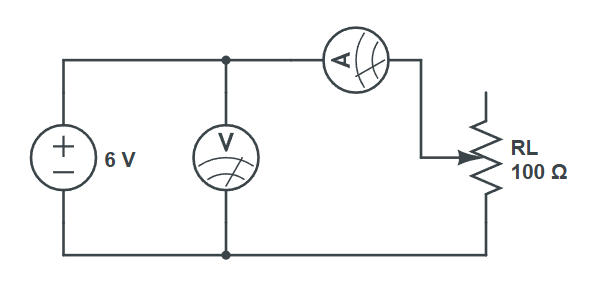
\includegraphics[width=0.3\textwidth]{fig1a.png}}\hspace{5mm}
            \subfloat[实际电压源测量]{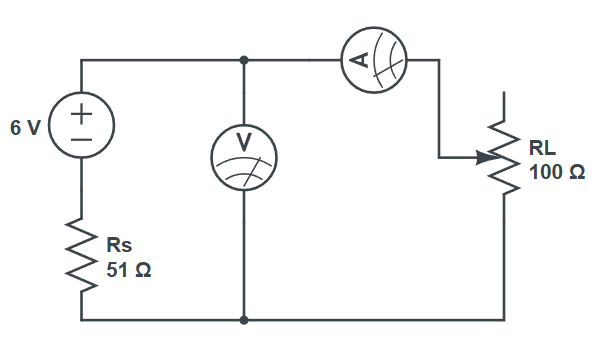
\includegraphics[width=0.3\textwidth]{fig1b.png}}
        \end{figure}\par
        测量结果如下:\par
        \begin{table}[!ht]
            \centering\begin{tabular}{c c c c c c c c}\toprule
                $R_L (\unit{\ohm})$ & 开路 & 600 & 500 & 400 & 300 & 200 & 100 \\ \midrule
                $U (\unit{\V})$ & 6 & 6.0019 & 6.0017 & 6.0013 & 6.0014 & 6.0010 & 5.9992 \\
                $I (\unit{\mA})$ & 0 & 10.048 & 12.084 & 15.078 & 19.875 & 26.57 & 60.4 \\ \bottomrule
            \end{tabular}\caption{理想电压源测量数据}
        \end{table}\par
        \begin{table}[!ht]
            \centering\begin{tabular}{c c c c c c c c}\toprule
                $R_L (\unit{\ohm})$ & 开路 & 600 & 500 & 400 & 300 & 200 & 100 \\ \midrule
                $U (\unit{\V})$ & 6 & 5.528 & 5.441 & 5.318 & 5.123 & 4.779 & 3.976 \\
                $I (\unit{\mA})$ & 0 & 9.254 & 10.953 & 13.358 & 17.173 & 23.908 & 39.845 \\ \bottomrule
            \end{tabular}\caption{实际电压源测量数据}
        \end{table}\par
        \begin{figure}[!ht]
            \caption{电压源的外特性曲线}
            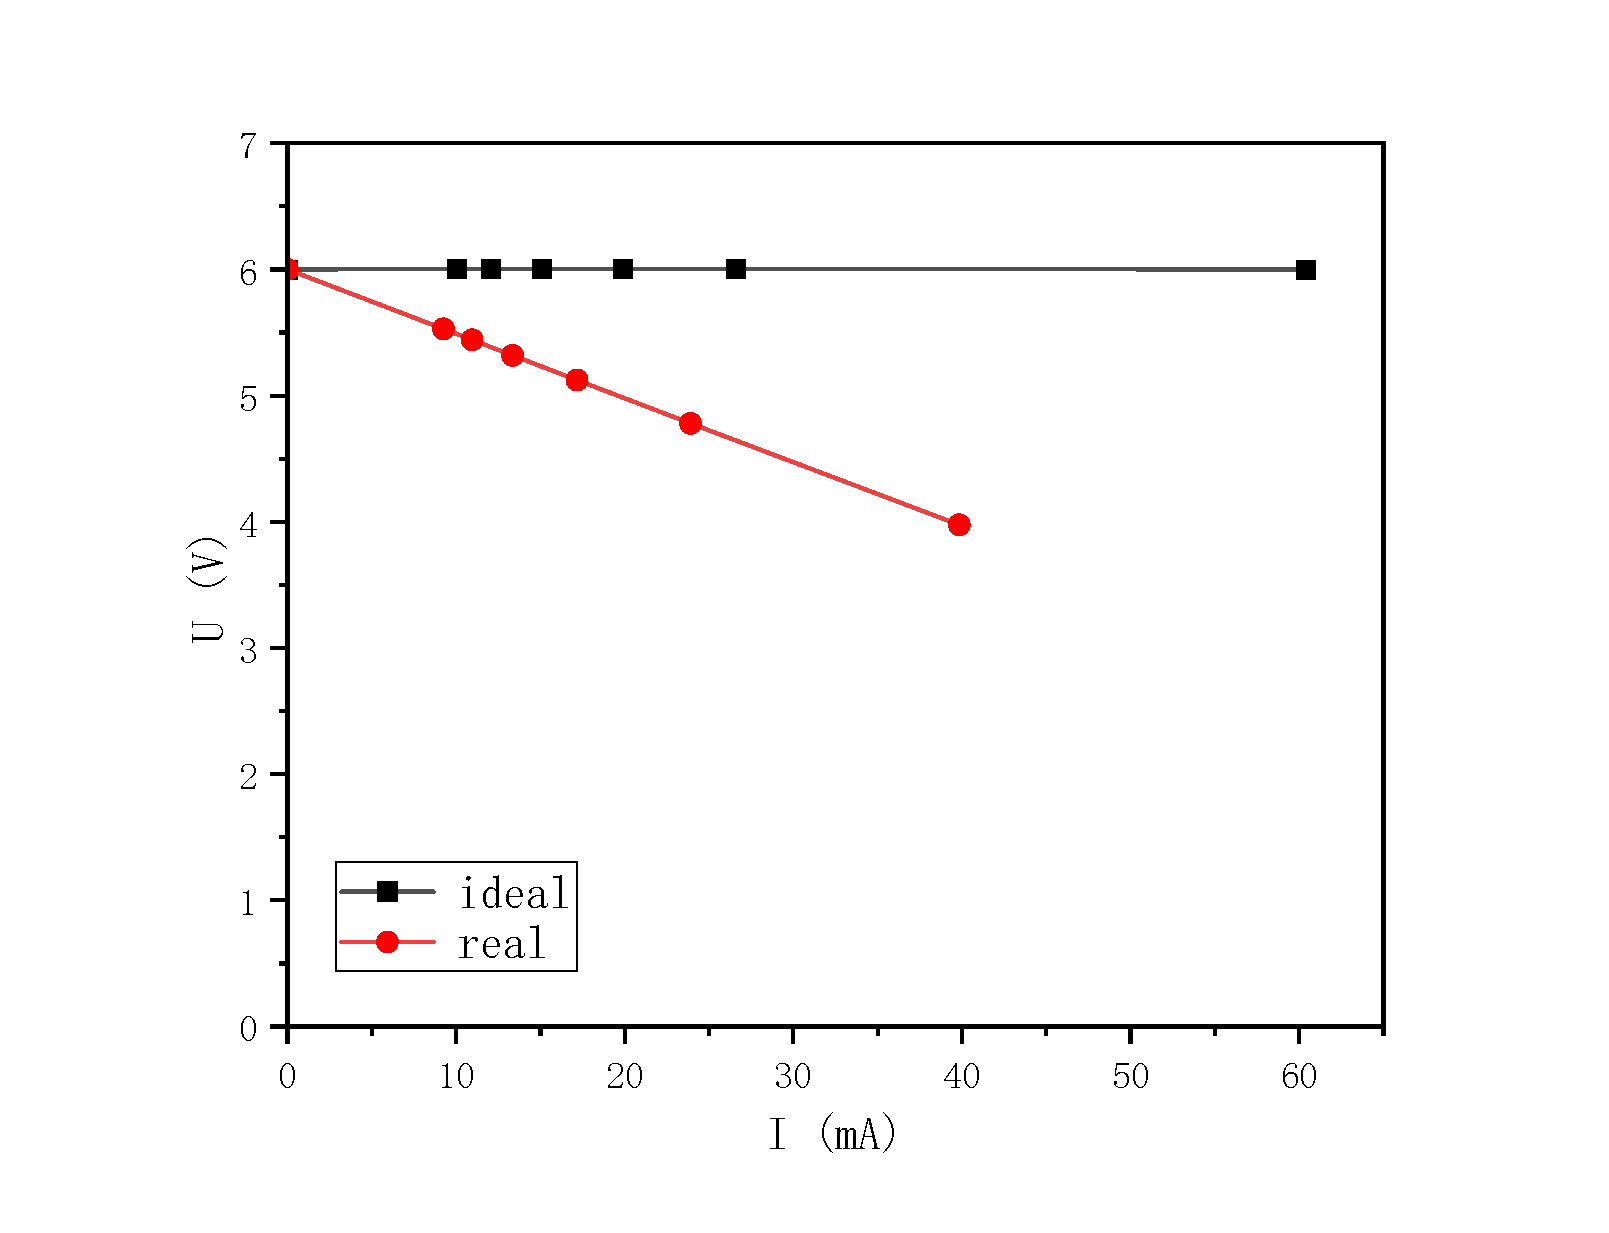
\includegraphics[width=0.45\textwidth]{fig2.pdf}
        \end{figure}\par
        可见,非理想电压源的电压会随着输出电流的增大逐渐降低,其本质是内阻分压满足欧姆定律 $U=IR$,总电流越大,内阻分压越多。\newpage


    \subsection{测定电流源的外特性}
        分别采用了以下两种电路接法:\par
        \begin{figure}[!ht]
            \subfloat[理想电流源测量]{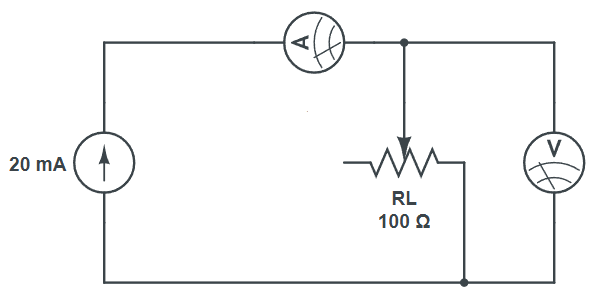
\includegraphics[width=0.3\textwidth]{fig3a.png}}\hspace{5mm}
            \subfloat[实际电流源测量]{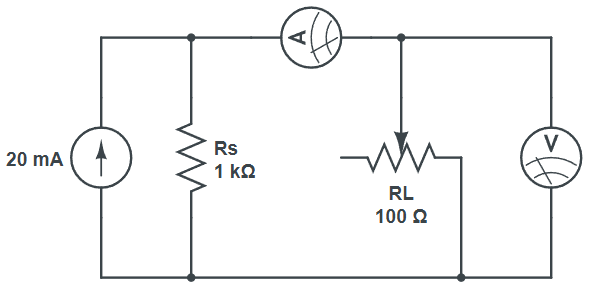
\includegraphics[width=0.3\textwidth]{fig3b.png}}
        \end{figure}\par
        测量结果如下:\par
        \begin{table}[!ht]
            \centering\begin{tabular}{c c c c c c c c}\toprule
                $R_L (\unit{\ohm})$ & 600 & 500 & 400 & 300 & 200 & 100 & 0 \\ \midrule
                $I (\unit{\mA})$ & 20.222 & 20.280 & 20.303 & 20.328 & 20.340 & 20.356 & 20.402 \\
                $U (\unit{\V})$ & 12.078 & 10.050 & 8.066 & 6.034 & 4.031 & 2.006 & 0 \\ \bottomrule
            \end{tabular}\caption{理想电流源测量数据}
        \end{table}\par
        \begin{table}[!ht]
            \centering\begin{tabular}{c c c c c c c c}\toprule
                $R_L (\unit{\ohm})$ & 600 & 500 & 400 & 300 & 200 & 100 & 0 \\ \midrule
                $I (\unit{\mA})$ & 13.183 & 14.116 & 15.147 & 16.362 & 17.730 & 19.371 & 21.333 \\
                $U (\unit{\V})$ & 7.920 & 7.004 & 6.020 & 4.854 & 3.513 & 1.909 & 0 \\ \bottomrule
            \end{tabular}\caption{实际电流源测量数据}
        \end{table}\par
        \begin{figure}[!ht]
            \caption{电流源的外特性曲线}
            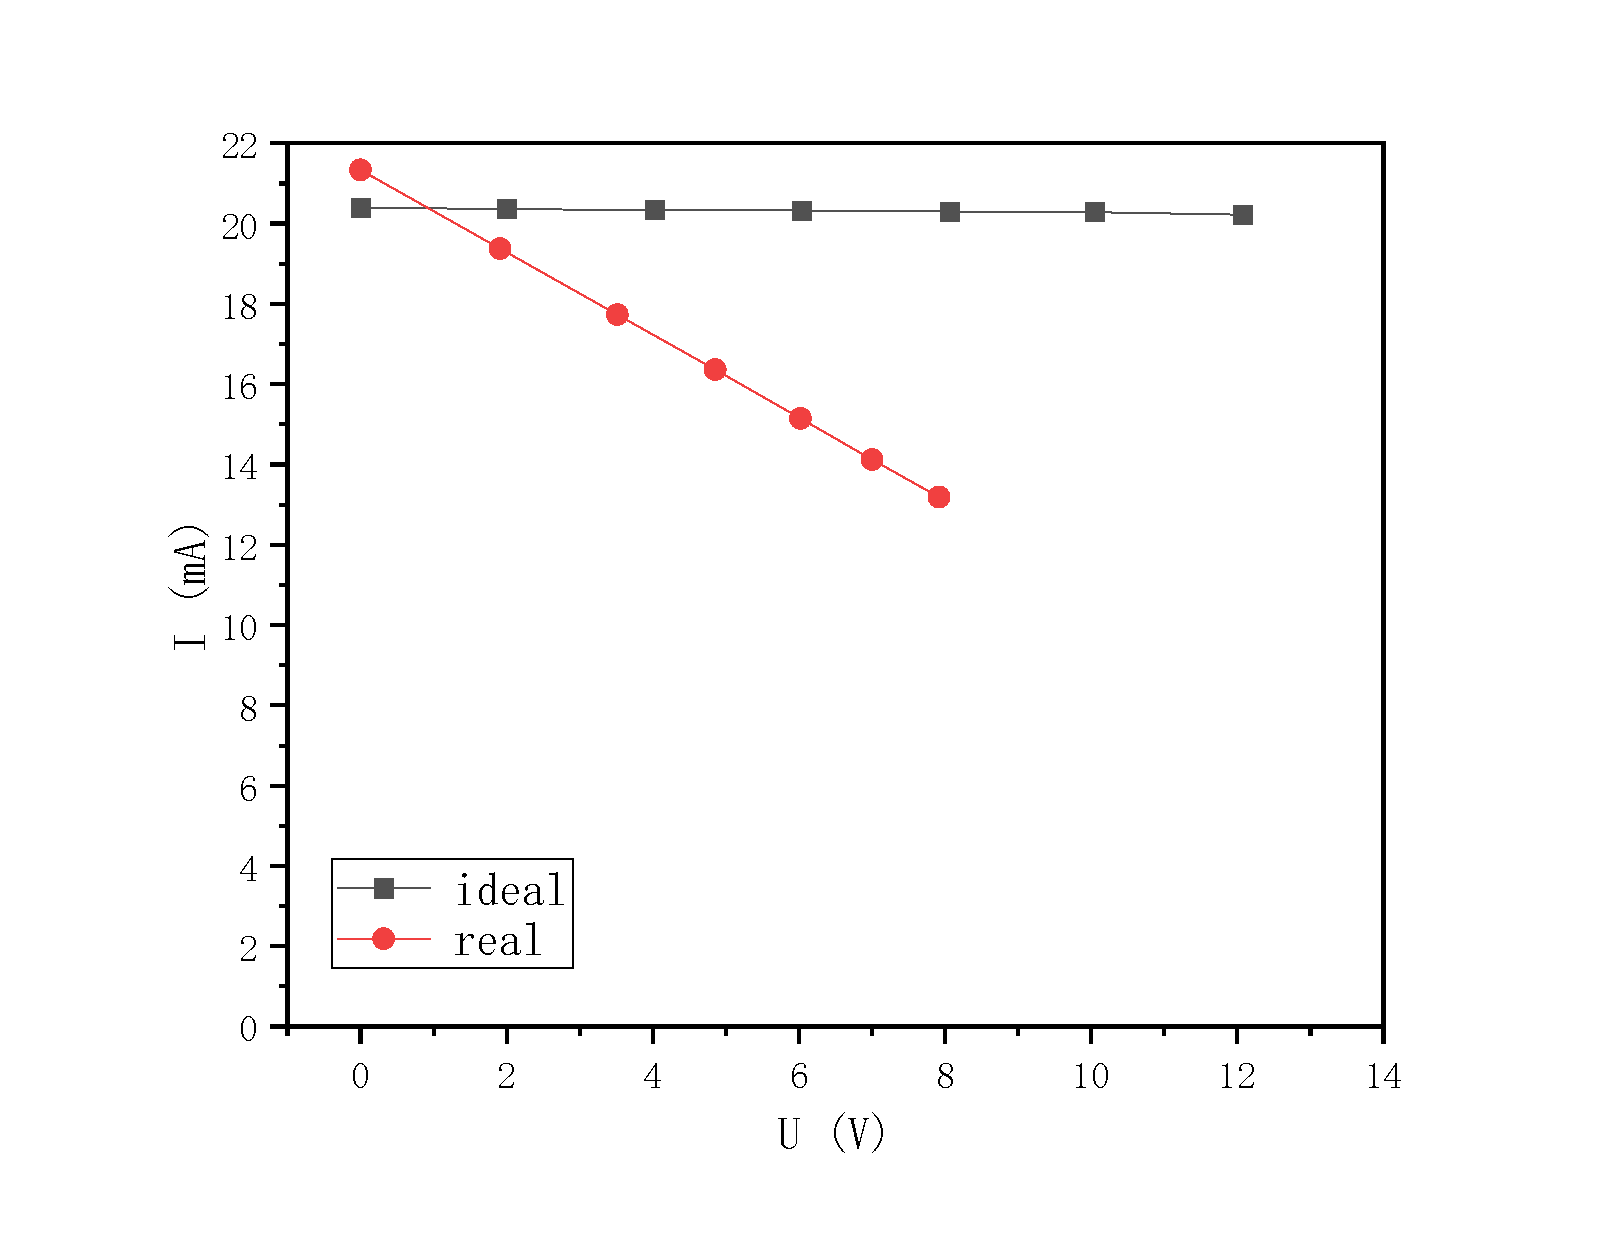
\includegraphics[width=0.45\textwidth]{fig4.pdf}
        \end{figure}\par
        虽然两条外特性曲线的起点不一致,但考虑到电流源调输出时确实不能输出与设定值完全一致的电流,所以只考虑两条曲线的变化趋势。与电压源的外特性曲线变化类似,实际电流源的输出电流会随着端口电压的增大而减小,其本质即为与理想电流源并联的电阻随电压增大,分流增多,干路电流便会减小。\newpage
    \subsection{测定电源等效变换的条件} 
        \begin{table}[!ht]
            \centering\begin{tabular}{|c | c|}\hline
                电流源供电时$U (\unit{\V})$ & 1.910  \\\hline
                电流源供电时$I (\unit{\mA})$ & 9.532 \\\hline
                保持读数不变时所需的电压源$U_s (\unit{\V})$ & 2.398 \\ \hline
            \end{tabular}\caption{等效变换条件测量}
        \end{table}\par
        由于使用的电流源可能有些接触不良,输出电流并不能稳定在 50 mA ,因此我重新采集了46.9 mA时的数据,根据电源等效变换的公式:$U_s=I_s R_s$
        \begin{align*}
            LHS&=2.398 \unit{\V} \\
            RHS&=46.9\unit{\mA} \times 51\unit{\ohm}=2.391 \unit{\V}\\
            \text{相对误差}&=0.29 \%
        \end{align*}

        误差分析:本次实验所采用的仪器精度很高,实验结果所包含的误差中,仪器误差占比较小,并且从实验结果可以看到,此次实验测量的误差都很小,可以认为是实验操作较规范。其余具体的误差来源如下:
        \begin{enumerate}
            \item 实验采用的电压/流源只是近似为理想源,实际上也会有内阻影响
            \item 实验箱上的待测元件与标称值本身存在误差,且长时间放置也会产生变化
            \item 测试线路上的电阻、寄生电容
            \item 测试当天的温度湿度导致的误差
            \item 引脚可能生锈而产生额外变化
        \end{enumerate}
   
\section{实验心得}
    本次实验测量了电压源和电流源的外特性曲线,还验证了电源转换的条件。虽然在验证电源转换的条件这个实验上并没有一次成功,而是隔周重新做了一次实验,但原理的正确性不会随着数值变化而变化,依然得到了正确的结果。
\newpage
\section{原始数据}
    \begin{figure}[!ht]
        \includegraphics*[width=0.9\textwidth]{data.jpg}
    \end{figure}
\end{document}